\documentclass[titlepage,twopage]{article}

\usepackage{graphicx}
\usepackage{hyperref}

\newcommand{\rarrow}{$\rightarrow$}

\title{Guide Map to Learn a Programming Language Generated by Crowd Insights}
\author{Mihai Codoban \and Caius Brindescu \and Semih Okur \and Kyungho Lee \and Shuo Yuan}

\begin{document}

\maketitle

\section*{Document history}

\begin{tabular}{| l | l | p{8cm} |}
\hline
\textbf{Date} & \textbf{Author} & \textbf{Comments} \\ \hline \hline
February 28, 2013 & Lee & Wrote the first draft, consulted with Prof. Bailiey \\ \hline 
February 28, 2013 & Lee & Put 3 figures to explain our concept \\ \hline
February 31, 2013 & Mihai & Added tool description \\ \hline
March 4, 2013 & Janus & Added Related Work section \\ \hline
March 4, 2013 & Mihai & Added reference \cite{mayer1981psychology} and detailed it at the start of section~\ref{sec:prelim-work}\\ \hline
March 5, 2013 & Semih & Detailed the map function and added reference \cite{okur2012developers} \\ \hline
March 5, 2013 & Caius & Made \LaTeX{} version \\ \hline
\end{tabular}

\cleardoublepage

\section{Project Summary}

Many people struggle with learning a programming language to create digital artifacts. Due to difficulties that people experience from programming, people might lose an opportunity to contribute to express their creativity for evolutionary innovations toward the society. In this regard, this research aims to design a creativity support tool for generating a �guide map to learn a programming language� made by valuable insights from crowds -- people who already experienced the same problems and learning process.

This research aims to:
\begin{itemize}
\item Observe students and teaching assistants (CS major, Art and Design major) to find major difficulties to learn a programming language in terms of learning process.
\item Find diverse opportunities to design an appropriate interface, which is functioning as a map for learning, for people (both of novices and experts).
\item Conduct crowdsourcing through online and offline to get sufficient insights, processes, tips, and useful resources to generate a map from diverse perspectives and backgrounds.
\item Build infrastructures and interfaces that enable people to engage and get real insights from a map generated by crowds so that the accelerate their learning process
\item Measure performances, conduct a post interview and analyze the results through a statistical methods to analyze the goal, objectives and impact of the tool 
\end{itemize}

\section{Project Description}

\begin{quote}
``Everybody in this country should learn how to program a computer because it teaches you how to think'' -- Steve Jobs
\end{quote}

A video, ``What most schools don't teach,'' circled the Internet this week. In it, a stream of renowned figures in the software world, such as, Microsoft, Dropbox, Facebook, and Twitter, make a compelling case for why everyone should learn how to program. This clip once again stresses the importance of programming; authors consider creating through programming is a vibrant way of expressing creativity in this generation \cite{winslow1996programming}.

Researchers in the science education field regard the behavior of programmers and get results from them as an information problem solving process that involves cognitive and metacognitive issues; they believe that programming techniques and skills that are not easily acquired \cite{lazonder2008information}.   

Unfortunately, most of people who have not sufficient background in the science or engineering would drop out of learning programming when they get stuck in a certain phase of their journey; those frustrating experiences prevent people from creating valuable artifacts or enabling evolutionary innovations \cite{pane1996usability}.

There are several reasons that hinder people from effective and efficient learning how to program. According to survey, one of biggest challenge for people to learn programming languages is a lack of understanding about an overall concept of the programming language that they wanted to use. The other challenges that they encounter are building functions and looping them within their program. After that, people would struggle with using libraries and input/output handling  \cite{lahtinen2005study}.

Another research also shows that these problematic experiences were observed not only within students whose background is not science or engineering but also happened for students whose major is computer science. (Murphy et al., 2006) It clearly shows that learning programming is not easy. Upon this, we empirically know that many novice programmers get lost in their way when they try to learn a new programming language by themselves \cite{milne2002difficulties}.

In this regard, we will design a creativity support tool that provides a guide map for people to get a holistic concept of the language so that they accelerate in learning a programming language by avoiding common pitfalls; the map will be generated by crowds� participation so that we could collect valuable insights, common pitfalls to avoid, useful links, source code and so forth. This project is initiated based on four what-if questions:
\begin{enumerate}
\item What if we can get a big picture including orthodox characteristics of a certain programming language in order to get a whole concept of the language?
\item What if we can expect hindrances that many people experienced before so that we can invest sufficient time to resolve issues rather than dropping out?
\item What if we can have shortcuts and bookmarks to answers to most problematic, cumbersome issues or questions while programming?
\item What if novices or experts can contribute to the other�s meta-learning process by drawing a big-picture letting them know what further steps are?
\end{enumerate}

\subsection{Design tenets}

\begin{itemize}
\item a programmer should quickly have access to previous explorations he has done. We do not want him to google the same concepts over and over again. Our tool should track the programmer�s learning progress so he can quickly revisit past concepts.
\item a programmer should not be assaulted with so much information that it becomes meaningless to him. He should receive suggestions that are most pertinent for the language topic he is currently exploring. Moreover, he should be able to refine, keep and collate only the suggestions he finds useful.
\item a programmer should be able to search and refine. He should be able to search different sources for hints, theory and practical explanation for different language concepts (SO, delicious etc). He should then be able to refine and retrieve concrete and diverse code examples that detail the particular topic (GitHub, SF etc)
\item a programmer should also receive help for the particular context he is coding in. The tool should be able to retrieve patterns of the code under edit and retrieve previously explored topics that deal with that code. Thus, the programmer can have the option to tailor searching and refining for the code under edit.
\end{itemize}

\section{Preliminary work}
\label{sec:prelim-work}

Many visualization system have been developed over the past years to help people learning programming language. By using computer graphics, workflow chart, and animation to help illustrate and present computer programs, processes, and algorithms.

\subsection{Jeliot 3 \cite{moreno2004visualizing}}

Jeliot 3 is a Program Visualization application. It visualizes how a Java program is interpreted. Method calls, variables, operation are displayed on a screen as the animation goes on, allowing the student to follow step by step the execution of a program. Programs can be created from scratch or they can be modifyed from previously stored code examples. The Java program being animated does not need any kind of additional calls, all the visualization is automatically generated. Jeliot 3 understands most of the Java constructs and it is able to animate them. Especial effort is currenlty being addressed to animate object oriented features, such as inheritance.

\begin{figure}[h!tb]
	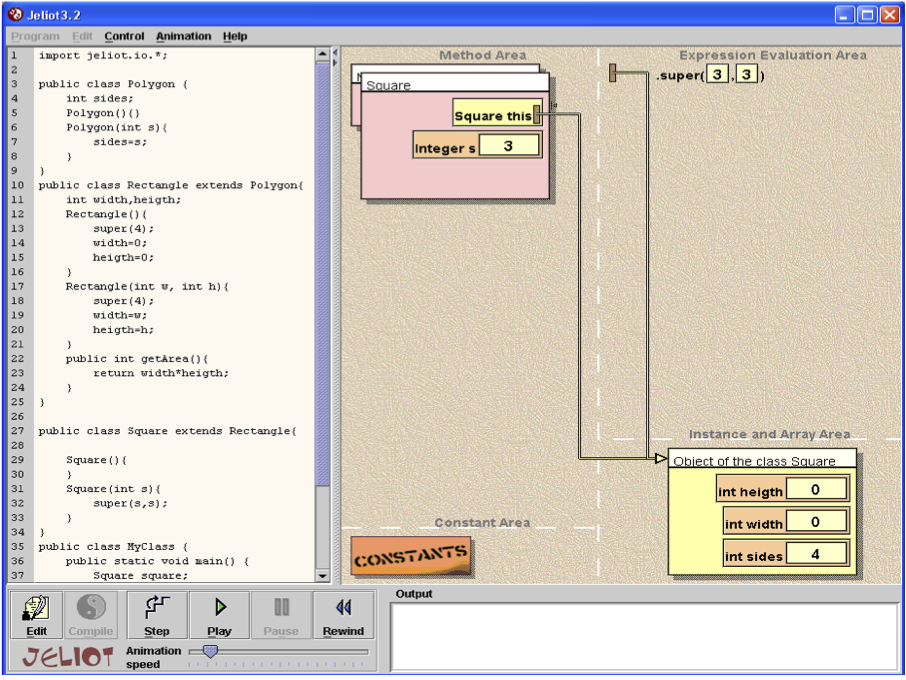
\includegraphics[width=\textwidth]{jeliot3.png}
\caption{Jeliot program interface}
\label{fig:jeliot3}
\end{figure}

Much research has been conducted on how people learn to program, and many techniques have been proposed.It seems that there are two approaches \cite{mayer1981psychology} which can deeply enhance learning: concrete models and personal models.

It has been shown that people who are presented with a concrete, simple model of the larger concept they are about to learn can gain a quicker understanding and retain much more than people who are deprived of such a model.

It has also been shown that people who are encouraged to make their own personal model of the concept they are learning, �putting things in one�s words�,  gain a much deeper understanding than people who do not undertake such activities.

By drawing insight from the above concepts, we present a tool that aids the programmer in learning, understanding, exploring and recalling a new programming language. On one hand the tool can present the hot topics of a particular programming language, as mined from the collective knowledge of online platforms such as Stack Overflow, Delicious or Github. On the other hand it allows the programmer to construct a unique mental model that represents that programmer�s unique learning journey. 

\subsection{Tool description}

Enable the programmer to build a personalized map, similar in form to the below examples,, that tracks his learning progress through a new language or concept. The programmer uses this map to search for and refine new knowledge and to keep track of all the concepts and related documents so far.

Advanced programmers can use this map as a continuous syntax reminder, instead of googling the same examples over and over again. The novice programmer can also use this map to document more theoretical knowledge such as basic algorithms and code idioms (eg: how to filter or aggregate collections by using loops).

Thus we can see two main functions of this map: to store knowledge in a structured form and to search for similar or new knowledge.

In terms of \emph{storing knowledge}, each node in the map would contain several documents. These are tutorials, forum questions and code snippets that helped the programmer in the past. In this manner, he does not have to spend time looking for the same examples over and over again.

Another important concept in terms of storing knowledge is that the map retains only what the programmer finds useful, only what he wants to keep for later reference. How does a programmer know whether to persist or not? Usually he does not know initially what is important (problem addressed below). This knowledge comes when he finds himself searching for the same concept more than once. Of course, this manner of growing the map is unique to every person.

In terms of \emph{searching for similar or new knowledge}, there would be two main approaches to grow the map: searching online places such Stack Overflow, Delicious or Github and suggestions based on similar maps from other users.

When searching online, the map tries to find similar hot topics related to the current context: For example, let�s say that the current map selection is Python \rarrow{} Sets. The map could then suggest hot topics related to Python sets by searching popular tags on Delicious or SO. It could find examples for set operations or set traversals. Python \rarrow{} Lists \rarrow{} Traversal would hopefully show different ways to traverse a list.

The map could also make suggestions of new map relations, nodes and documentation based on similar maps from other users.

In the end, we would also like to take this map into the IDE and let it suggest help according to the context under edit. While coding, the programmer could ask help about the current context. The map could either find the required knowledge in its structure (it has been previously searched by the programmer) or it could search help platforms and code repositories for questions, tutorials and code snippets most similar to code under edit.

\subsection{Steps}

Since this is a big project, we shall implement it in steps, as detailed below.

\subsubsection{Programming language map}

\textbf{High probability to be finished during course project}

Code search have always been essential to software development; it is the cornerstone of activities such as program comprehension and maintenance. In this step, we will introduce learn-by-code and learn-by-questions technologies. 

The first stage would be to build the map of hot topics concerning a particular programming language. We shall use Stack Overflow and Delicious to find these hot topics. In this manner we use the accumulated knowledge of the crowd to find what is important and difficult for that particular language.

Both platforms have web services through which we can retrieve popular tags.

To guide the search we need a seed of important concepts that detail the main elements of programming languages (ex: statement, decision, iteration, function, class, inheritance etc). To find these seeds we shall review literature involving learning  programming languages. We shall also conduct interviews with both novice and experienced programmers.

These seed concepts will act as a scaffold on which our map is built. We will use them to bootstrap the web platform search. 

Programming language map will function like a cheat sheet which will dynamically change based on your code snippets. All these information in the map will not be visible to the developers during coding process. When the developer introduces some concepts into the code, the related nodes will be shown up in our map. For instance, if the developer did not extend any class, he will not see information and code snippets related with inheritance.

In overall, the map will have 2 different modes. First mode enables developers to introduce new concepts (e.g., array iteration, inheritance) with simple code snippets. These code snippets will come from our previously mined repositories \cite{okur2012developers}. Second mode will enable developers to explore advanced topics through our information map mined from Stack Overflow and Delicious. 

\subsubsection{Customize the map}
\textbf{Medium probability to be finished during course project.}

The above maps are centered around a particular programming language. They are not unique or personalized to the user.

In this phase we would like to let the user customize the map. He should be able to add or delete nodes that he is not interested in. He should also be able to edit nodes by deleting and adding documentation of his own (notes, code snippets, urls, tutorials etc)

The map should be able to reconstruct itself it by populating the nodes added by the user.

\subsubsection{Map mimics the learning progress}
\textbf{Medium to low probability to be finished during course project.}

The map should grow with the user. He could start with a single node, let�s say ``Python''. He should get suggestions according to the concept seeds in order to guide him, if he wishes so.

He should be able to add new nodes of his own accord and retrieve information and documentation specific for that particular node in the map.

\subsubsection{Plug into IDE}
\textbf{Low probability to be finished during course project.}

The map can live inside the IDE to offers help according to the code context under edit.

\subsection{A feel of what should be}

Three design prototypes are presented in figures \ref{fig:map1}, \ref{fig:map2} and \ref{fig:map3}.

\begin{figure}[hbt]
	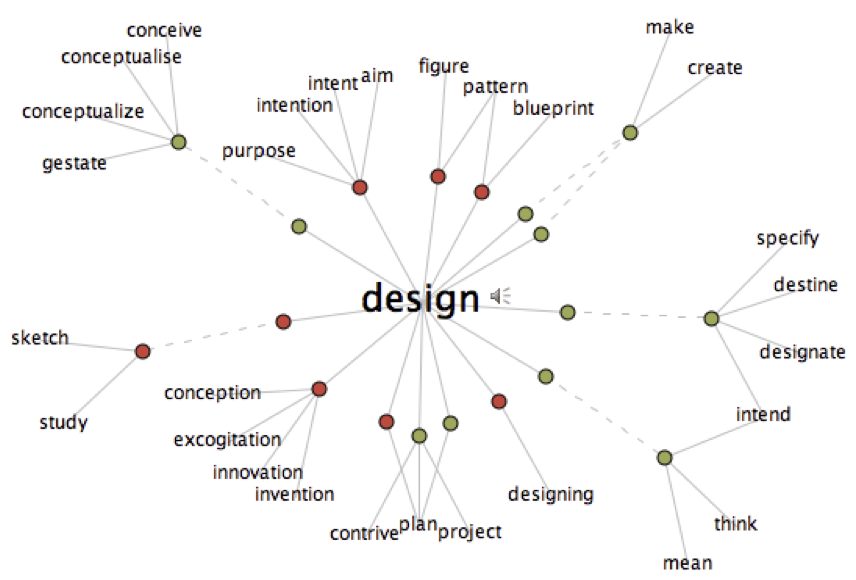
\includegraphics[width=\textwidth]{map1.png}
\caption{Design protype 1}
\label{fig:map1}
\end{figure}

\begin{figure}[hbt]
	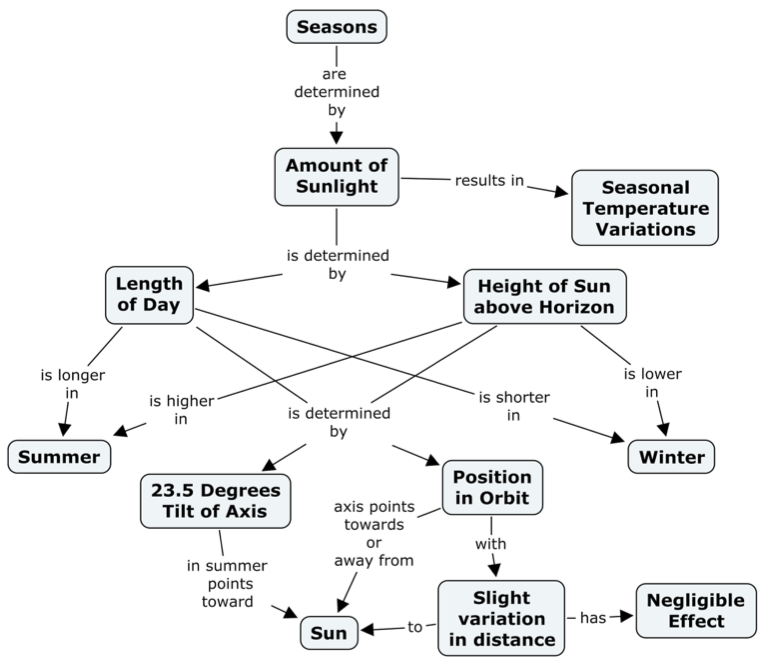
\includegraphics[width=\textwidth]{map2.png}
\caption{Design protype 2}
\label{fig:map2}
\end{figure}

\begin{figure}[hbt]
	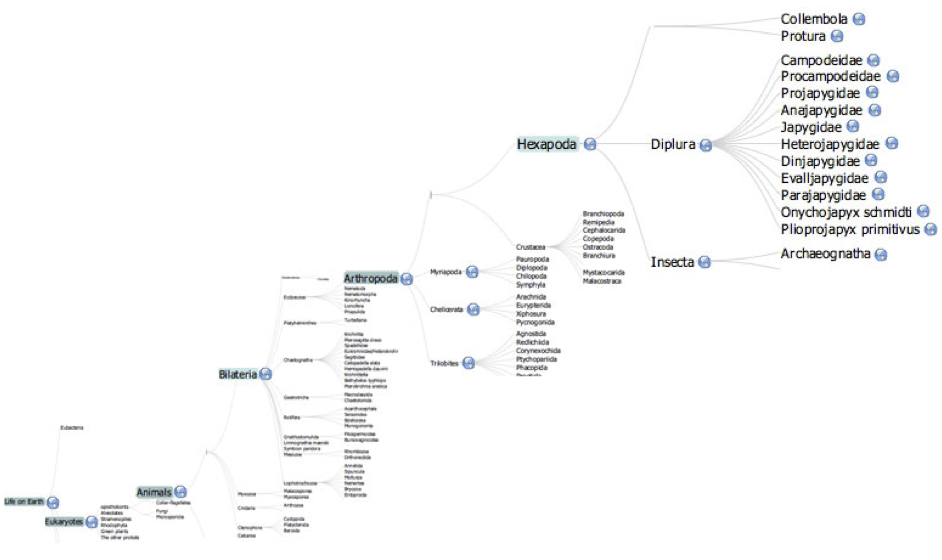
\includegraphics[width=\textwidth]{map3.png}
\caption{Design protype 3}
\label{fig:map3}
\end{figure}

\clearpage

\section{Methods}

Mostly will use the well-known and effect design methods such as
\begin{itemize}
\item \hyperref[1]{http://socialinnovation.typepad.com/silk/silk-method-deck.html}
\item \hyperref[2]http://www.ideo.com/work/method-cards
\end{itemize}

\section{Time schedule}

\begin{table}[hbt]
\begin{tabular}{| l |p{6.5cm} | p{5cm} |}
\hline
\textbf{Date} & \textbf{Tasks} & \textbf{Deliverables} \\
\hline \hline
February 28 & Consult with Professor Bailey. Report to IRB. & Proposal revision \\ \hline
March 5 & W1: Interview(Consult) with Experts & Interview Report \\ \hline
March 7 & W2: Field Research & Insight Report \\ \hline
March 12 & W3: User Research & Insight Report \\ \hline
March 14 & W4: Concept Design: Goals, Persona and Ideation & Paper Prototype \\ \hline
March 19 & SPRING BREAK & - \\ \hline
March 21 & SPRING BREAK & - \\ \hline
March 26 & W5: Prototyping and Iteration 2; Consult with Prof. Bailey & Storyboard(Wireframe)
or \newline Working prototype \\ \hline
March 28 & W6: Self reflection & Project progress report \\ \hline
April 2 & W7: Implementation and Iteration 1 & UI design \\ \hline
April 4 & W8: Implementation and Iteration 2, Crowdsourcing 1 & Sourcecode, HIT results \\ \hline
April 9 & W9: Implementation and Iteration 3, Crowdsourcing 2 & Sourcecode, HIT results \\ \hline
April 11 & W10: Usability Test, Post User Interview & Experiment report \\ \hline
April 16 & W11: Statistical analysis and Discussion & Analysis Report \\ \hline
April 18 & W12: Write the final paper	 & Final paper draft \\ \hline
April 23 & Project presentations, Peer-review and revise 1 & Final paper revision 1 \\ \hline
April 25 & Project presentations, Peer-review and revise 2 & Final paper revision 2  \\ \hline
May 1 & Final Paper due & Final paper submit \\ \hline
\end{tabular}
\end{table}

\clearpage

\nocite{brand2005information}
\nocite{deek1999common}
\nocite{lahtinen2005study}
\nocite{lazonder2008information}
\nocite{murphy2006women}
\nocite{fincher1999we}
\nocite{pane1996usability}
\nocite{robins2003learning}
\nocite{soloway1989studying}
\nocite{winslow1996programming}
\nocite{mayer1981psychology}
\nocite{okur2012developers}

\bibliographystyle{plain}
\bibliography{proposal.bib}

\end{document}